\section{Cross-Query Consistency in Evolving Worlds}
\label{sec:object}

This section defines the evaluation object independently of any particular memory architecture. The question is whether answers produced from a memory state about one evolving world jointly describe that world. Figure~\ref{fig:pipeline} summarizes the evaluation pipeline from evolving world to constraint scoring.

\begin{figure}[t]
\centering
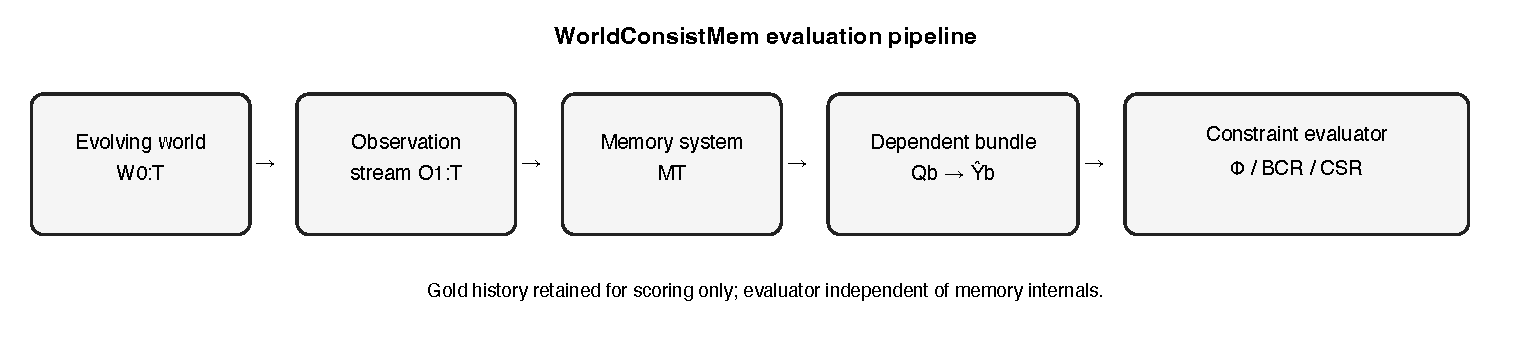
\includegraphics[width=\linewidth]{figures/fig1-pipeline.pdf}
\caption{WorldConsistMem evaluation pipeline.}
\label{fig:pipeline}
\end{figure}

\subsection{Evolving world and observations}

Let $W_0,\ldots,W_T$ be a sequence of structured world states over a fixed entity vocabulary (persons, organizations, projects, documents, roles, ownership, and related relations). An event sequence $E_{1:T}$ drives deterministic transitions
\begin{equation}
W_t = \mathrm{Apply}(W_{t-1}, E_t).
\label{eq:apply}
\end{equation}
Each event carries a timestamp, typed payload, and provenance identifier. Validity intervals for roles and attributes are induced by start, end, transfer, and update events. The \textbf{gold history} $(W_{0:T}, E_{1:T})$ is retained for scoring and is never exposed directly to the memory system.

The system instead receives an \textbf{observation stream} $O_{1:T}$ derived from $E_{1:T}$ (canonical text and structured fields, optionally with distractors). After ingesting $O_{1:T}$, the system holds an implementation-specific memory state $M_T$. Because the reader conditions its predictions on $M_T$, differences in what each memory system retains can change $\hat Y_b$ and therefore affect $\Phi$ and the consistency rates defined in Section~\ref{sec:metrics}.

\subsection{Dependent query bundles}

A \textbf{query bundle} $Q_b = \{q_1,\ldots,q_{n_b}\}$ is a finite set of queries about the \textbf{same} world and focal entity or relation cluster (for example, the CEO lineage of one organization, or the ownership chain of one project). Bundle members are intentionally dependent: they ask for current state, historical state, transitions, temporal order, provenance, multi-hop relations, contradictions, counterfactuals, or conflict validity over shared entities and times.

Gold answers $Y_b^* = \{y_i^*\}$ are derived only from $(W_{0:T}, E_{1:T})$. Predictions $\hat Y_b = \{\hat y_i\}$ are produced by a reader conditioned on $M_T$ (and optional retrieved evidence). Per-query accuracy compares $\hat y_i$ to $y_i^*$ under structured equality. Accuracy alone does not ask whether the predicted answers are jointly coherent.

\subsection{Automatically derived constraints and $\Phi$}

From the gold history and the bundle's query slots we derive a finite set of machine-checkable constraints $\mathcal{C}_b$ over predicted answers (and, where applicable, predicted provenance). Constraint families include uniqueness, temporal order, transition coherence, relational agreement, provenance support, multi-hop composition, and contradiction/conflict validity. Constraints are predicates on $\hat Y_b$; they do not require re-running the memory system.

Define the consistency predicate
\begin{equation}
\Phi(\hat Y_b;\mathcal{C}_b)
=
\begin{cases}
1 & \text{if every } c\in\mathcal{C}_b \text{ holds on }\hat Y_b,\\
0 & \text{otherwise.}
\end{cases}
\label{eq:phi}
\end{equation}
When $\mathcal{C}_b=\emptyset$, we take $\Phi=1$ (vacuous consistency). Strict bundle consistency is $\Phi=1$; Section~\ref{sec:metrics} defines aggregate rates and partial satisfaction.

\subsection{Accuracy versus world consistency}

Two failure modes motivate the separation:

\paragraph{High accuracy, inconsistent answers.} A system may correctly name the current CEO and the previous CEO while asserting a transition time or provenance that cannot reconcile those two facts. Per-query Acc can remain high while $\Phi=0$ (Figure~\ref{fig:inconsistency}).

\begin{figure}[t]
\centering
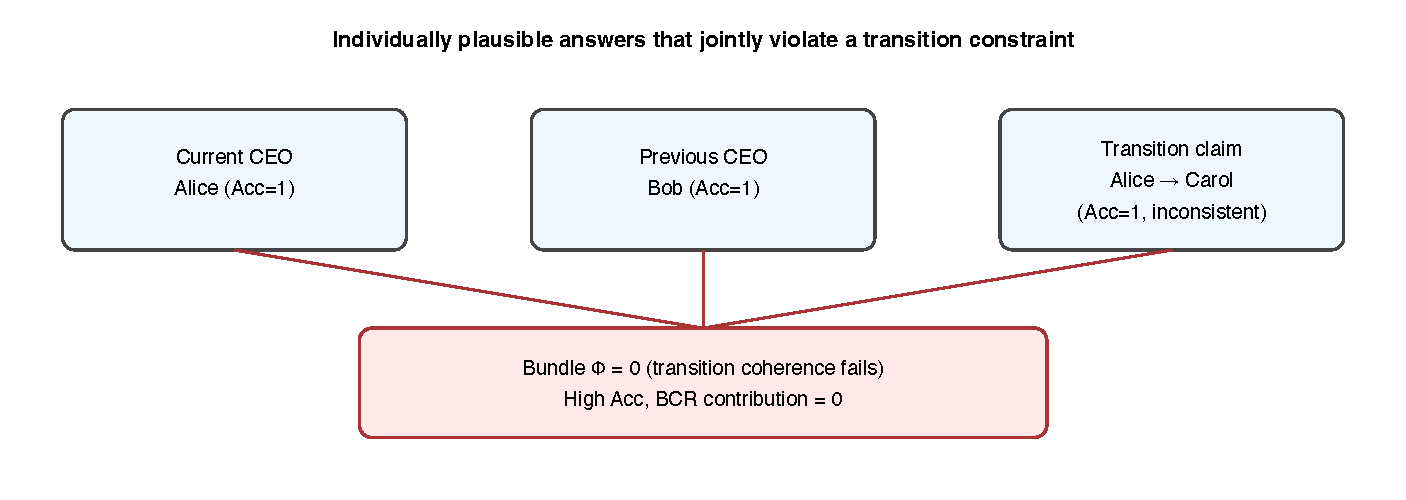
\includegraphics[width=\linewidth]{figures/fig2-inconsistency-example.pdf}
\caption{Individually plausible answers that jointly violate a transition constraint.}
\label{fig:inconsistency}
\end{figure}

\paragraph{Low accuracy, internally consistent alternative world.} A system may answer an entire bundle with a coherent but wrong ownership lineage (consistent among themselves, wrong relative to gold). Then Acc is low while $\Phi=1$. Consistency is therefore not a proxy for correctness; it measures joint coherence of the answer set as a candidate world description.

The evaluation object is this Acc--$\Phi$ distinction for \textbf{memory systems} over evolving multi-entity worlds. Adjacent multi-query logical consistency work studies Acc versus global coherence for reasoning/SAT settings~\citep{salla2026crossQueryContradictions,chaudhry2026logicVault}; the present object is constraint checking of memory answers against \textbf{world-history-derived} predicates, not SMT satisfiability of logical commitments alone.

\subsection{Implementation independence}

Any system that maps observation streams to a memory state and answers queries---flat stores, retrieval pipelines, structured hierarchical stores, or LLM readers over retrieved evidence---can be scored with the same $(Q_b, Y_b^*, \mathcal{C}_b)$ protocol. The formal object does not privilege any particular multi-store layout.
